\documentclass[12pt,a4paper]{article}
\usepackage[margin=2.5cm]{geometry}
\usepackage{amsmath,amssymb}
\usepackage{booktabs}
\usepackage{array}
\usepackage{enumitem}
\usepackage{parskip}
\usepackage[T1]{fontenc}
\usepackage{times}
\usepackage{tikz}
\usetikzlibrary{positioning,arrows.meta,shapes.geometric}

\setlength{\parindent}{0pt}
\setlength{\parskip}{6pt}
\setlist[itemize]{noitemsep, topsep=2pt, leftmargin=1.4em, label={--}}
\setlist[enumerate]{noitemsep, topsep=2pt, leftmargin=1.8em}

\begin{document}

\begin{center}
{\Large\textbf{IE 400 -- Term Project Report}}\\[4pt]
Spring 2026
\end{center}

\bigskip

%=======================================================================
\section*{\underline{Question 1: Museum Escape}}

\subsection*{Problem Definition}

Lara starts at cell $(1,1)$ and must reach the exit at cell $(8,8)$ on an
$8\times 8$ grid in the minimum number of time steps. At each time step she may move
one cell up, down, left, or right, or stay in place. She cannot enter obstacle cells.
Three security cameras patrol the museum; if Lara occupies any camera-visible cell at
the same time step, she is caught.

\textbf{Obstacle cells:} $(1,8),\,(2,3),\,(2,7),\,(3,6),\,(4,1),\,(4,2),\,(4,8),\,(5,6),\,(6,4),\,(7,3),\,(7,4),\,(7,5)$

\subsection*{Camera Movement Tables}

\textbf{Camera 1} (period~4, horizontal patrol along row~3):

\begin{center}
\begin{tabular}{cccc}
\toprule
$t$ & Position & Direction & Visible Cells \\
\midrule
0   & $(3,3)$ & Right & $(3,3),(3,4),(3,5)$ \\
1   & $(3,4)$ & Right & $(3,4),(3,5),(3,6)$ \\
2   & $(3,5)$ & Left  & $(3,5),(3,4),(3,3)$ \\
3   & $(3,4)$ & Left  & $(3,4),(3,3),(3,2)$ \\
$4+$ & \multicolumn{3}{l}{repeats from $t=0$} \\
\bottomrule
\end{tabular}
\end{center}

\textbf{Camera 2} (period~6, middle corridor):

\begin{center}
\begin{tabular}{cccc}
\toprule
$t$ & Position & Direction & Visible Cells \\
\midrule
0 & $(4,6)$ & Down  & $(4,6),(5,6)$ \\
1 & $(5,6)$ & Down  & $(5,6),(6,6)$ \\
2 & $(6,6)$ & Right & $(6,6),(6,7)$ \\
3 & $(6,7)$ & Left  & $(6,7),(6,6)$ \\
4 & $(6,6)$ & Up    & $(6,6),(5,6)$ \\
5 & $(5,6)$ & Up    & $(5,6),(4,6)$ \\
$6+$ & \multicolumn{3}{l}{repeats from $t=0$} \\
\bottomrule
\end{tabular}
\end{center}

\textbf{Camera 3} (period~4, exit area diagonal):

\begin{center}
\begin{tabular}{cccc}
\toprule
$t$ & Position & Direction & Visible Cells \\
\midrule
0 & $(7,7)$ & NE & $(7,7),(6,8)$ \\
1 & $(6,8)$ & SW & $(6,8),(7,7),(8,6)$ \\
2 & $(7,7)$ & SW & $(7,7),(8,6)$ \\
3 & $(8,6)$ & SW & $(8,6),(7,7),(6,8)$ \\
$4+$ & \multicolumn{3}{l}{repeats from $t=0$} \\
\bottomrule
\end{tabular}
\end{center}

The combined camera-visible set at time $t$ is
\[
  F(t) \;=\; C_1[t \bmod 4]\;\cup\; C_2[t \bmod 6]\;\cup\; C_3[t \bmod 4].
\]

%-----------------------------------------------------------------------
\subsection*{Task 1: Integer Programming Formulation}

\textbf{Sets and Parameters}

\begin{itemize}
  \item $\mathcal{V}$: set of all non-obstacle cells $(r,c)$, where $r,c\in\{1,\ldots,8\}$
  \item $N(r,c)$: set of cells reachable in one step from $(r,c)$, i.e.\ $(r,c)$ and its orthogonal
        neighbours that lie in $\mathcal{V}$
  \item $F(t)$: set of cells visible by any camera at time $t$
  \item $T$: planning horizon (total number of steps); to be minimised
\end{itemize}

\textbf{Decision Variables}

\[
  x_{t,r,c} \in \{0,1\} \qquad t=0,1,\ldots,T,\quad (r,c)\in\mathcal{V}
\]
$x_{t,r,c}=1$ if Lara occupies cell $(r,c)$ at time step $t$, and $0$ otherwise.

\textbf{Objective Function}
\[
  \min\; T
\]

\textbf{Constraints}

\textbf{(C1) Initial position:}
\[
  x_{0,1,1}=1, \qquad x_{0,r,c}=0 \quad \forall\,(r,c)\in\mathcal{V},\;(r,c)\neq(1,1)
\]

\textbf{(C2) One cell per time step:}
\[
  \sum_{(r,c)\in\mathcal{V}} x_{t,r,c}=1 \qquad \forall\;t=0,1,\ldots,T
\]

\textbf{(C3) Valid movement:}
\[
  x_{t+1,r,c}\;\leq\!\!\sum_{(r',c')\in N(r,c)}\!\! x_{t,r',c'}
  \qquad \forall\;t=0,\ldots,T-1,\quad(r,c)\in\mathcal{V}
\]

\textbf{(C4) Camera avoidance:}
\[
  x_{t,r,c}=0 \qquad \forall\;t,\quad\forall\,(r,c)\in F(t),\quad(r,c)\neq(8,8)
\]
The exit cell $(8,8)$ is exempt: Lara may step there even if a camera sees it.

\textbf{(C5) Exit reached at horizon $T$:}
\[
  x_{T,8,8}=1
\]

\textbf{(C6) Binary domain:} $x_{t,r,c}\in\{0,1\}$

%-----------------------------------------------------------------------
\subsection*{Task 2: Base Case}

A time-expanded BFS is run first over the state space $\{(r,c,t)\}$ to determine the minimum
horizon $T^*$. Because every step has unit cost, BFS is guaranteed to find the shortest path.
The IP is then solved at $T=T^*$ with Gurobi to confirm the result.

\medskip
\textbf{Result:} $T^*=16$ steps. The optimal path is:

\begin{center}
\begin{tabular}{cc|cc|cc}
\toprule
$t$ & Cell & $t$ & Cell & $t$ & Cell \\
\midrule
 0 & $(1,1)$ &  6 & $(2,5)$ & 12 & $(6,7)$ \\
 1 & $(1,2)$ &  7 & $(3,5)$ & 13 & $(6,7)$ \\
 2 & $(1,2)$ &  8 & $(4,5)$ & 14 & $(6,8)$ \\
 3 & $(1,3)$ &  9 & $(5,5)$ & 15 & $(7,8)$ \\
 4 & $(1,4)$ & 10 & $(6,5)$ & 16 & $(8,8)$ \\
 5 & $(1,5)$ & 11 & $(6,6)$ & & \\
\bottomrule
\end{tabular}
\end{center}

Lara waits at $(1,2)$ during $t=1,2$ to let Camera~1 clear the corridor, then proceeds
straight to the exit. All constraints (C1)--(C6) are verified to be satisfied.

%-----------------------------------------------------------------------
\subsection*{Task 3: Booby Trap}

\textbf{Additional rule:} if Lara visits cell $(5,1)$, she may never visit cell $(8,3)$
afterwards.

This is an if-then implication. We introduce a cumulative binary variable
\[
  y_t \in \{0,1\}, \qquad t=0,1,\ldots,T,
\]
where $y_t=1$ means Lara has visited $(5,1)$ at or before time $t$. The linearisation is:
\begin{align*}
  y_t &\;\geq\; x_{t,5,1} && \forall\;t \tag{trap triggered}\\
  y_t &\;\geq\; y_{t-1}   && \forall\;t\geq 1 \tag{stays triggered}\\
  x_{t,8,3} &\;\leq\; 1-y_{t-1} && \forall\;t\geq 1 \tag{block $(8,3)$ after trap}
\end{align*}

\textbf{Result:} $T^*=16$ steps, same path as the base case. The base-case path never visits
$(5,1)$, so the booby-trap constraint is satisfied trivially and the optimal cost does not
increase.

%-----------------------------------------------------------------------
\subsection*{Task 4: Exit Lock ($t<18$)}

\textbf{Additional rule:} the cells
$\mathrm{LOCKED}=\{(6,7),(7,6),(7,7),(8,6),(6,8)\}$
are forbidden before $t=18$:
\[
  x_{t,r,c}=0 \qquad \forall\;t<18,\quad(r,c)\in\mathrm{LOCKED}.
\]

\textbf{Result:} $T^*=20$ steps. Lara must detour through the interior and wait until
$t=18$ when the exit area becomes accessible.

\begin{center}
\begin{tabular}{cc|cc|cc}
\toprule
$t$ & Cell & $t$ & Cell & $t$ & Cell \\
\midrule
 0 & $(1,1)$ &  8 & $(5,3)$ & 16 & $(5,7)$ \\
 1 & $(1,2)$ &  9 & $(5,4)$ & 17 & $(5,8)$ \\
 2 & $(1,2)$ & 10 & $(4,4)$ & 18 & $(6,8)$ \\
 3 & $(2,2)$ & 11 & $(4,5)$ & 19 & $(7,8)$ \\
 4 & $(3,2)$ & 12 & $(4,5)$ & 20 & $(8,8)$ \\
 5 & $(3,3)$ & 13 & $(4,6)$ & & \\
 6 & $(4,3)$ & 14 & $(4,7)$ & & \\
 7 & $(5,3)$ & 15 & $(5,7)$ & & \\
\bottomrule
\end{tabular}
\end{center}

%-----------------------------------------------------------------------
\subsection*{Task 5: Ghost Checkpoint ($t=3$)}

\textbf{Additional rule:} Lara must occupy cell $(4,4)$ at exactly $t=3$:
\[
  x_{3,4,4}=1.
\]

\textbf{Result: Infeasible.} A BFS on the obstacle map (ignoring cameras) shows that the
minimum number of steps to reach $(4,4)$ from $(1,1)$ is~6. Since the constraint requires
arrival at $t=3<6$, it is geometrically impossible regardless of the path chosen. The model
has no feasible solution.

%-----------------------------------------------------------------------
\subsection*{Task 6: Branch and Bound (Base Case)}

\textbf{LP Relaxation.}
The LP relaxation of the IP is obtained by replacing $x_{t,r,c}\in\{0,1\}$ with
$x_{t,r,c}\in[0,1]$. The LP optimal value gives a lower bound on the IP optimal value. If
the LP optimum happens to be integer, it is also optimal for the IP.

\textbf{Algorithm.}
B\&B builds an enumeration tree. At each node~$j$:

\begin{enumerate}
  \item Solve the LP relaxation of the subproblem. Let $z^{\mathrm{LP}}(j)$ denote its value.
  \item \textbf{Case~1 (Infeasibility):} $z^{\mathrm{LP}}(j)=-\infty$. Fathom node~$j$.
  \item \textbf{Case~2 (Bounding):} $\lfloor z^{\mathrm{LP}}(j)\rfloor \leq z^I$. Fathom
        node~$j$; no descendant can improve the incumbent $z^I$.
  \item \textbf{Case~3 (Integrality):} $z^{\mathrm{LP}}(j)>z^I$ and the LP solution is
        integer. Update incumbent $z^I\leftarrow z^{\mathrm{LP}}(j)$. Fathom node~$j$.
  \item \textbf{Case~4 (Branching):} $z^{\mathrm{LP}}(j)>z^I$ but the solution is
        fractional. Select the most-fractional variable $x_{t^*,r^*,c^*}$ and create two
        children: one adds $x_{t^*,r^*,c^*}=0$, the other adds $x_{t^*,r^*,c^*}=1$.
\end{enumerate}

Node selection uses \textbf{best-first} order (process the active node with the largest
$z^{\mathrm{LP}}$). The algorithm terminates when no active nodes remain.

\textbf{Application to the Museum IP.}
Since $T$ is fixed at $T^*=16$ by BFS, the IP is a feasibility problem. The LP relaxation
is highly constrained by the movement and camera constraints, so fractional variables are
rare. B\&B terminates within very few branching levels and confirms the optimal path with
$T^*=16$.

\medskip
\begin{center}
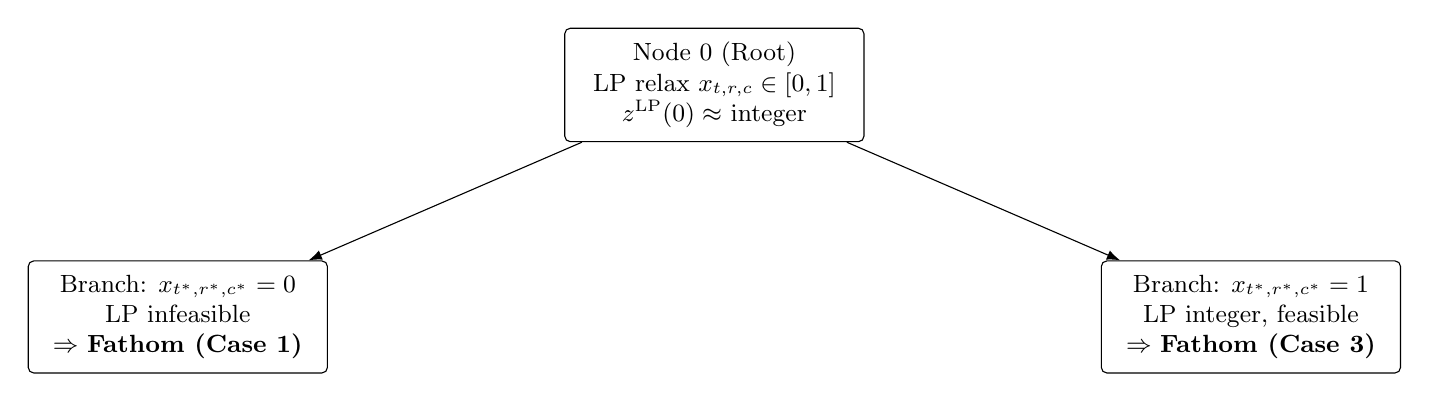
\begin{tikzpicture}[
  node distance=15mm and 30mm,
  every node/.style={draw, rounded corners=2pt, align=center,
                     font=\small, inner sep=5pt, minimum width=38mm},
  arr/.style={-Latex}
]
\node (root) {Node 0 (Root)\\LP relax $x_{t,r,c}\in[0,1]$\\$z^{\mathrm{LP}}(0)\approx$ integer};
\node (L) [below left=of root]  {Branch: $x_{t^*,r^*,c^*}=0$\\LP infeasible\\$\Rightarrow$ \textbf{Fathom (Case 1)}};
\node (R) [below right=of root] {Branch: $x_{t^*,r^*,c^*}=1$\\LP integer, feasible\\$\Rightarrow$ \textbf{Fathom (Case 3)}};
\draw[arr] (root) -- (L);
\draw[arr] (root) -- (R);
\end{tikzpicture}
\end{center}

\medskip
The right child yields the same integer path found by BFS, confirming $T^*=16$ as optimal.

\newpage

%=======================================================================
\section*{\underline{Question 2: CCI Production Planning}}

\subsection*{Problem Definition}

Coca-Cola \.{I}\c{s}ecek (CCI) plans production at two plants -- Ankara~(A) and
Istanbul~(I) -- over $m=1,\ldots,6$ months. The objective is to minimize the total cost of
inventory holding, cross-region transportation, workforce wages, hiring, layoffs, and
bottling-mode switching, subject to demand, capacity, workforce, and cross-shipping
constraints.

\subsection*{Data}

\textbf{Monthly demand} $d_{jm}$ (million liters, ML), where $j\in\{W,\,CE\}$:

\begin{center}
\begin{tabular}{lcccccc}
\toprule
Region $j$ & $m=1$ & $m=2$ & $m=3$ & $m=4$ & $m=5$ & $m=6$ \\
\midrule
Western (W)             & 9 & 9 & 14 & 12 & 12 & 13 \\
Central \& Eastern (CE) & 7 & 7 &  8 &  9 &  8 &  9 \\
\bottomrule
\end{tabular}
\end{center}

\textbf{Plant parameters}, where $i\in\{A,\,I\}$:

\begin{center}
\begin{tabular}{lll}
\toprule
Parameter & Ankara ($i=A$) & Istanbul ($i=I$) \\
\midrule
Bottling rate, 2\,L & $6{,}000$ bot/hr $=12{,}000$ L/hr & $9{,}000$ bot/hr $=18{,}000$ L/hr \\
Bottling rate, 1\,L & $10{,}000$ bot/hr $=10{,}000$ L/hr & $15{,}000$ bot/hr $=15{,}000$ L/hr \\
Available hours/month & 720 & 720 \\
Initial workforce $w_{i0}$ & 60 & 100 \\
Primary region & CE & W \\
\bottomrule
\end{tabular}
\end{center}

\textbf{Cost parameters:}
\begin{itemize}
  \item Wage: $c_w = 1{,}200$ TL per employee per month
  \item Hiring: $c_h = 1{,}500$ TL per new employee
  \item Layoff: $c_l = 2{,}000$ TL per laid-off employee
  \item Inventory holding: $c_{\text{inv}} = 0.05$ TL/L/month $= 50{,}000$ TL/ML/month
  \item Cross-region transport: $c_{\text{tr}} = 0.10$ TL/L $= 100{,}000$ TL/ML
  \item Bottling-mode switching: $c_{\text{sw}} = 20{,}000$ TL per plant per month
\end{itemize}

\textbf{Policy parameters:}
$\alpha=0.25$ (cross-ship cap),
$\beta=0.10$ (safety-stock fraction),
$\Delta=10$ (max workforce change per period).

\subsection*{Decision Variables}

All production and inventory quantities are in million liters (ML).
Indices: $i\in\{A,I\}$ for plant, $j\in\{W,CE\}$ for region, $m\in\{1,\ldots,6\}$ for month.

\begin{itemize}
  \item $p_{i,k,m}\geq 0$ \quad production of bottle size $k\in\{1\text{L},2\text{L}\}$
        at plant $i$ in month $m$ (ML)
  \item $s_{i,j,m}\geq 0$ \quad supply shipped from plant $i$ to region $j$ in month $m$ (ML)
  \item $I_{i,m}\geq 0$ \quad end-of-month inventory at plant $i$ in month $m$ (ML)
  \item $w_{i,m}\in\mathbb{Z}_{\geq0}$ \quad packaging workforce at plant $i$ in month $m$
  \item $h_{i,m},\,l_{i,m}\in\mathbb{Z}_{\geq0}$ \quad employees hired / laid off at plant $i$
        in month $m$
  \item $\delta_{i,k,m}\in\{0,1\}$ \quad equals 1 if bottle size $k$ is produced at plant $i$
        in month $m$
  \item $z_{i,m}\in\{0,1\}$ \quad equals 1 if both bottle sizes are produced at plant $i$ in
        month $m$ (switching indicator)
\end{itemize}

For compactness we also write: $p^1_{i,m}=p_{i,1\text{L},m}$, $p^2_{i,m}=p_{i,2\text{L},m}$;
and the primary region of plant $A$ is $CE$, of plant $I$ is $W$.

\subsection*{Objective Function}

\[
\min\; Z = C_{\text{inv}}+C_{\text{tr}}+C_w+C_h+C_l+C_{\text{sw}}
\]
\begin{align*}
C_{\text{inv}} &= 50{,}000\sum_{i}\sum_{m} I_{i,m} \\
C_{\text{tr}}  &= 100{,}000\!\!\!\sum_{\substack{i,j:\,j\neq \text{primary}(i)}}\sum_{m} s_{i,j,m} \\
C_w            &= 1{,}200\sum_{i}\sum_{m} w_{i,m} \\
C_h            &= 1{,}500\sum_{i}\sum_{m} h_{i,m} \\
C_l            &= 2{,}000\sum_{i}\sum_{m} l_{i,m} \\
C_{\text{sw}}  &= 20{,}000\sum_{i}\sum_{m} z_{i,m}
\end{align*}

\subsection*{Constraints}

\textbf{(D1) Bottling capacity} (total bottling hours $\leq 720$ per plant per month):
\[
  \frac{p^2_{A,m}\cdot10^6}{12{,}000}+\frac{p^1_{A,m}\cdot10^6}{10{,}000}\leq720,
  \qquad
  \frac{p^2_{I,m}\cdot10^6}{18{,}000}+\frac{p^1_{I,m}\cdot10^6}{15{,}000}\leq720
  \qquad\forall\,m
\]

\textbf{(D2) Packaging capacity} (total production $\leq$ workforce capacity):
\[
  p^1_{i,m}+p^2_{i,m}\;\leq\;0.1\,w_{i,m} \qquad\forall\,i,\,m
\]

\textbf{(D3) Workforce balance} ($w_{A,0}=60$, $w_{I,0}=100$):
\[
  w_{i,m}=w_{i,m-1}+h_{i,m}-l_{i,m} \qquad\forall\,i,\,m
\]

\textbf{(D4) Workforce smoothing} ($\Delta=10$):
\[
  w_{i,m}-w_{i,m-1}\leq 10, \qquad w_{i,m-1}-w_{i,m}\leq 10 \qquad\forall\,i,\,m
\]
(These two inequalities linearise $|w_{i,m}-w_{i,m-1}|\leq10$.)

\textbf{(D5) Inventory balance} (initial inventories $=0$):
\[
  I_{i,m}=I_{i,m-1}+p^1_{i,m}+p^2_{i,m}-\sum_{j}s_{i,j,m} \qquad\forall\,i,\,m
\]

\textbf{(D6) Demand fulfillment} (no backlogging):
\[
  \sum_{i}s_{i,j,m}\;\geq\;d_{j,m} \qquad\forall\,j,\,m
\]

\textbf{(D7) Cross-shipping cap} ($\alpha=25\%$):
\[
  s_{i,j,m}\;\leq\;\alpha\,d_{j,m}
  \qquad\forall\,i,\,m,\;\text{where }j\neq\text{primary}(i)
\]

\textbf{(D8) Safety stock} ($\beta=10\%$, months $m=1,\ldots,5$):
\[
  I_{i,m}\;\geq\;\beta\,d_{j^*(i),\,m+1} \qquad m=1,\ldots,5
\]
where $j^*(i)$ is the primary region of plant $i$.

\textbf{(D9) Zero ending inventory} (perishability after month 6):
\[
  I_{i,6}=0 \qquad\forall\,i
\]

\textbf{(D10) Bottling-mode switching cost} (big-$M=50$ ML):
\[
  p^k_{i,m}\;\leq\;50\,\delta_{i,k,m} \qquad\forall\,i,\,k,\,m
\]
\[
  z_{i,m}\;\geq\;\delta_{i,1\text{L},m}+\delta_{i,2\text{L},m}-1 \qquad\forall\,i,\,m
\]
$z_{i,m}=1$ if and only if both bottle sizes are produced at plant $i$ in month $m$,
which triggers the $20{,}000$ TL switching cost.

\subsection*{Gurobi Results}

The MILP was solved with Gurobi. All constraints were verified to hold.

\medskip
\textbf{Optimal Total Cost: $Z^*=2{,}168{,}800$ TL}

\medskip
\textbf{Cost breakdown:}

\begin{center}
\begin{tabular}{lr}
\toprule
Component & Cost (TL) \\
\midrule
Inventory holding      & $600{,}000$ \\
Cross-region transport & $70{,}000$ \\
Wages                  & $1{,}414{,}800$ \\
Hiring                 & $72{,}000$ \\
Layoffs                & $12{,}000$ \\
Switching              & $0$ \\
\midrule
\textbf{Total}         & $\mathbf{2{,}168{,}800}$ \\
\bottomrule
\end{tabular}
\end{center}

\medskip
\textbf{Workforce decisions:}

\begin{center}
\begin{tabular}{crrrrrr}
\toprule
$m$ & $w_{A,m}$ & $h_{A,m}$ & $l_{A,m}$ & $w_{I,m}$ & $h_{I,m}$ & $l_{I,m}$ \\
\midrule
1 & 70 & 10 & 0 & 106 &  6 & 0 \\
2 & 74 &  4 & 0 & 112 &  6 & 0 \\
3 & 84 & 10 & 0 & 122 & 10 & 0 \\
4 & 86 &  2 & 0 & 121 &  0 & 1 \\
5 & 81 &  0 & 5 & 121 &  0 & 0 \\
6 & 81 &  0 & 0 & 121 &  0 & 0 \\
\bottomrule
\end{tabular}
\end{center}

\medskip
\textbf{Production and inventory decisions:}

\begin{center}
\begin{tabular}{crrrrrrrr}
\toprule
$m$ & $p^1_{A,m}$ & $p^2_{A,m}$ & $p^1_{I,m}$ & $p^2_{I,m}$
    & $I_{A,m}$ & $I_{I,m}$ & $s_{A,W,m}$ & $s_{I,CE,m}$ \\
\midrule
1 & 7.000 & 0.000 & 0.000 & 10.600 & 0.700 & 0.900 & 0.000 & 0.700 \\
2 & 7.200 & 0.000 & 0.000 & 11.200 & 0.800 & 3.000 & 0.000 & 0.000 \\
3 & 0.000 & 8.400 & 0.000 & 12.200 & 1.200 & 1.200 & 0.000 & 0.000 \\
4 & 0.000 & 8.600 & 0.000 & 12.100 & 0.800 & 1.200 & 0.000 & 0.000 \\
5 & 0.000 & 8.100 & 0.000 & 12.100 & 0.900 & 1.300 & 0.000 & 0.000 \\
6 & 0.000 & 8.100 & 0.000 & 11.700 & 0.000 & 0.000 & 0.000 & 0.000 \\
\bottomrule
\end{tabular}
\end{center}

\medskip
\textbf{Observations.}
\begin{itemize}
  \item No switching cost is incurred: each plant uses only one bottle size per month
        ($z_{i,m}=0$ for all $i,m$). Ankara uses 1\,L in months~1--2 then switches to 2\,L
        from month~3; Istanbul uses only 2\,L throughout.
  \item Cross-region shipping is minimal. Only Istanbul$\to$CE ships 0.700\,ML in month~1
        (within the $0.25\times7=1.75$ ML cap).
  \item Wages dominate the cost at $1{,}414{,}800$ TL ($\approx65\%$ of total), reflecting
        the labour-intensive packaging step.
  \item Safety stock constraints bind in months~1--5, driving the inventory levels observed.
\end{itemize}

\end{document}
